\documentclass[a4paper,11pt]{article} % screen setting

\usepackage[a4paper]{geometry}
\geometry{verbose,tmargin=1.5cm,bmargin=1.5cm,lmargin=1.5cm,rmargin=1.5cm}

\setlength{\parskip}{\smallskipamount}
\setlength{\parindent}{0pt}

%\usepackage{fontspec}
\usepackage[libertine]{newtxmath}
\usepackage[no-math]{fontspec}
\setmainfont{Linux Libertine O}
\setmonofont{DejaVu Sans Mono}

\usepackage{hyperref}
\usepackage{url}
\usepackage{xcolor}

% DARKMODE
%\pagecolor[rgb]{0,0,0} %black
%\color[rgb]{0.8,0.8,0.8} %grey

\usepackage{amsmath}
\usepackage{amssymb}

\usepackage{graphicx}
\usepackage{float}

\usepackage{minted}

\newminted{dart}{breaklines,fontsize=\footnotesize}
\newminted{bash}{breaklines,fontsize=\footnotesize}
\newminted{text}{breaklines,fontsize=\footnotesize}

\newcommand{\txtinline}[1]{\mintinline[breaklines,fontsize=\footnotesize]{text}{#1}}
\newcommand{\dartinline}[1]{\mintinline[breaklines,fontsize=\footnotesize]{python}{#1}}

\newmintedfile[pythonfile]{python}{breaklines,fontsize=\footnotesize}

\definecolor{mintedbg}{rgb}{0.90,0.90,0.90}
\usepackage{mdframed}
\BeforeBeginEnvironment{minted}{
    \begin{mdframed}[backgroundcolor=mintedbg,%
        topline=false,bottomline=false,%
        leftline=false,rightline=false]
}
\AfterEndEnvironment{minted}{\end{mdframed}}


\usepackage{setspace}

\onehalfspacing

\usepackage{appendix}


\newcommand{\highlighteq}[1]{\colorbox{blue!25}{$\displaystyle#1$}}
\newcommand{\highlight}[1]{\colorbox{red!25}{#1}}


\begin{document}


\title{Pemrograman User Interface dengan Flutter:\\
Navigasi dan Rute}
\author{Fadjar Fathurrahman}
\date{}
\maketitle

\section{Tujuan}

\begin{itemize}
\item mengenal dan menggunakan beberapa metode navigasi/rute ada aplikasi Flutter
\end{itemize}

\section{Navigasi dan Rute}
Hampir seluruh aplikasi yang kita gunakan pada divais akan memiliki lebih dari satu
halaman atau tampilan. Misalnya ketika kita mengklik suatu tombol maka kita akan
dibawa ke halaman lain. Pada aplikasi web, biasanya suatu halaman memiliki URL
yang mengindikasikan alamat suatu halaman. Alamat ini biasanya juga sering diistilahkan
dengan rute (\textit{route}). Pengembang aplikasi \textit{mobile} biasa menggunakan
istilah navigasi.

Pada Flutter terdapat empat cara untuk navigasi:
\begin{itemize}
\item Stacks: Setiap widget memenuhi seluruh layar. Pengguna menekan button untuk
berpindah dari suatu halaman ke halaman lain yang urutannya sudah ditentukan.
Histori tersimpan dan pengguna dapat kembali ke layar sebelumnya dengan menekan button
back.
\item Drawers: Biasanya terdapat pada bagian kiri, ketika user menekan suatu icon atau
melakukan swipe dari kiri ke kanan. Drawer biasanya mirip dengan menu.
\item Tabs: Sebagian ruang pada layar disisihkan untuk tab-tab yang berada pada bagian
atas atau bawah layar. Ketika tab ditekan, widget tertentu akan ditampilkan sesuai dengan
tab yang ditekan.
\item Dialog: mirip dengan pop-up window.
\end{itemize}


\section{Stacks}
Stack secara sederhana dapat dianalogikan seperti suatu tumpukan, misalkan tumpukan
buku. Kita dapat menambahkan buku baru dengan cara meletakkan buku tersebut pada
bagian atas tumpukan buku yang sudah ada. Operasi ini disebut dengan operasi \textit{push}.
Ketika kita ingin mengambil buku, makan buku pada tumpukan atas harus diambil terlebih dahulu.
Operasi ini disebut dengan operasi \textit{pop}.

Pada Flutter, konsep navigasi dengan stack mirip dengan tumpukan. Ketika pengguna
diberikan suatu tampilan atau halaman baru, Flutter akan melakukan operasi \textit{push},
yaitu menambahkan suatu widget di atas tumpukan, dan pengguna akan melihat widget tersebut.
Setiap kali kita melakukan operasi \textit{push} pada Flutter, kita menambahkan widget baru pada
bagian atas tumpukan. Jika kita ingin kembali ke tampilan sebelumnya, kita perlu
melakukan operasi \textit{pop}, yaitu menghilangkan widget terakhir dari tumpukan sehingga
yang terlihat adalah widget sebelumnya.

Pada Flutter, rute didefinisikan dengan cara memberikan rute tersebut nama. Nama rute
berupa string yang diawali dengan tanda \txtinline{/}, misalnya \txtinline{'/login'}.
Rute awal, yaitu tampilan yang pertama terlihat atau \textit{home} adalah \txtinline{'/'}.
Pendefinisian rute dilakukan pada level \txtinline{MaterialApp}. Contohnya:
\begin{dartcode}
Widget build(BuildContext context) {
  return MaterialApp(
    title: 'My App',
    initialRoute: '/',
    routes: {
      '/': (BuildContext ctx) => HomePage(),
      '/login': (BuildContext ctx) => LoginPage(),
      '/browse': (BuildContext ctx) => Browse(),
      '/products': (BuildContext ctx) => ViewProducts(),
      '/checkout': (BuildContext ctx) => Checkout(),
    }
  );
}
\end{dartcode}

Untuk melakukan navigasi pengguna ke suatu halaman secara manual, kita perlu
menggunakan \txtinline{Navigator}, yaitu dengan metode \txtinline{pushNamed(context,route)}
dan \txtinline{pop(context)}. Misalkan kita ingin menavigasi pengguna ke suatu route
ketika suatu button ditekan:
\begin{dartcode}
ElevatedButton(
  child: Text('Check out'),
  onPressed: () {
    Navigator.pushNamed(context, '/checkout');
  }
)
\end{dartcode}
Setelah pengguna selesai dan ingin kembali ke halaman sebelumnya dengan menekan button:
\begin{dartcode}
ElevatedButton(
  child: Text('Go back'),
  onPressed: () {
    Navigator.pop(context);
  }
)
\end{dartcode}
Jika aplikasi kita memiliki widget \txtinline{Scaffold}, maka kita juga dapat menggunakan
back arrow pada appbar di sebelah kiri atas untuk kembali ke halaman sebelumnya.

Contoh program:
\begin{dartcode}
import 'package:flutter/material.dart';

void main() => runApp(MyApp());

class MyApp extends StatelessWidget {
  @override
  Widget build(BuildContext context) {
    return MaterialApp(
      title: 'Navigasi Sederhana',
      theme: ThemeData(primarySwatch: Colors.green),
      routes: {
        '/': (BuildContext ctx) => FirstPage(),
        '/second': (BuildContext ctx) => SecondPage(),
      },
    );
  }  
}

class FirstPage extends StatelessWidget {
  @override
  Widget build(BuildContext context) {
    return Scaffold(
      appBar: AppBar(title: Text('First Page Title')),
      body: Center(
        child: Column(
          mainAxisAlignment: MainAxisAlignment.center,
          children: [
            Text('This is first page', style: TextStyle(fontSize: 20),),
            ElevatedButton(
              child: Text('Go to second page', style: TextStyle(fontSize: 20),),
              onPressed: () {
                Navigator.pushNamed(context, '/second');
              },
            ),
          ],
        ),
      ),
    );
  }
}
  
class SecondPage extends StatelessWidget {
  @override
  Widget build(BuildContext context) {
    return Scaffold(
      appBar: AppBar(title: Text('Second Page Title')),
      backgroundColor: Colors.blue,
      body: Center(
        child: Column(
          mainAxisAlignment: MainAxisAlignment.center,
          children: [
            Text('This is second page', style: TextStyle(fontSize: 20),),
            ElevatedButton(
              child: Text('Go back to first page', style: TextStyle(fontSize: 20)),
              onPressed: () {
                Navigator.pop(context);
              },
            ),
          ],
        ),
      ),
    );
  }
}
\end{dartcode}

Contoh tampilah program pada halaman pertama:

{\center
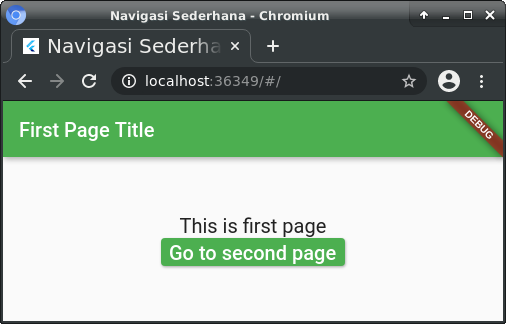
\includegraphics[scale=0.5]{images/navigation_named_01.png}
\par}

Tampilan halaman kedua, ketika tombol ditekan:

{\center
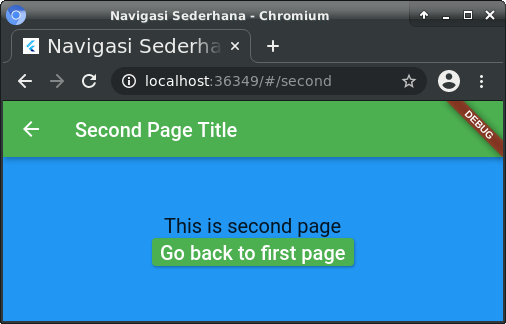
\includegraphics[scale=0.5]{images/navigation_named_02.png}
\par}


\section{Drawer}

Drawer biasanya digunakan jika kita memiliki banyak pilihan rute atau navigasi.
Pada website, drawer ini mirip dengan menu yang akan muncul jika suatu Icon (biasanya
disebut hamburger menu) ditekan. Ketika suatu pilihan pada menu ditekan kita dapat
melakukan navigasi pengguna ke suatu rute dengan menggunakan \txtinline{Navigator.push()}.

Pada Flutter, kita dapat menggunakan widget \txtinline{Drawer} yang dapat diberikan
pada properti \txtinline{drawer} dari suatu \txtinline{Scaffold}.
\begin{dartcode}
Widget build(BuildContext context) {
  return Scaffold(
    appBar: AppBar(title: Text('Drawer Navigation'),),
    body: Text('This is drawer navigation'),
    drawer: Drawer(
      child: ListView(
        children: [
          Text('Option 1'),
          Text('Option 2'),
          Text('Option 3'),
        ],
      ),
    ),
  )
}
\end{dartcode}

Biasanya kita ingin agar kita dapat mengakses drawer pada setiap halaman pada aplikasi.
Pada kasus tersebut, kita perlu membuat agar drawer yang dibuat dalam suatu kelas.
\begin{dartcode}
Widget build(BuildContext context) {
  return Scaffold(
    appBar: AppBar(title: Text('Drawer Navigation'),),
    body: Text('This is drawer navigation'),
    drawer: MyDrawer(),);
}

class MyDrawer extend StatelessWidget {
  // definisi ...
}
\end{dartcode}

Untuk mengisi menu pada drawer kita dapat menggunakan \txtinline{Column} atau
\txtinline{ListView}. Kita juga dapat menggunakan \txtinline{DrawerHeader} yang
dapat digunakan untuk menampilkan logo atau infomasi lain kepada user.
Contoh:
\begin{dartcode}
return Drawer(
  child: ListView(
    children: [
      DrawerHeader(
        child: Stack(
          children: [
            Image.asset('assets/images/logo.png'),
            Container(
              alignment: Alignment.bottomLeft,
              child: Text('My Logo'),
            ),
          ]
        ),
      ),
      ListTile(
        leading: Icon(Icons.home),
        title: Text('Home'),
        onTap: () {
          Navigator.pushNamed(context, '/');
        }
      ),
      // item lain ...
    ],
  ),
);
\end{dartcode}


Beriku ini adalah contoh program:
\begin{dartcode}
import 'package:flutter/material.dart';

void main() => runApp(MyApp());
  
class MyApp extends StatelessWidget {
  @override
  Widget build(BuildContext context) {
    return MaterialApp(
      title: 'Navigasi dengan Drawer',
      theme: ThemeData(primarySwatch: Colors.green),
      routes: {
        '/': (BuildContext ctx) => HomePage(),
        '/drawer1': (BuildContext ctx) => WidgetWithDrawer1(),
        '/drawer2': (BuildContext ctx) => WidgetWithDrawer2(),
        '/drawer3': (BuildContext ctx) => WidgetWithDrawer3(),
      },
    );
  }
}
  
class HomePage extends StatelessWidget {
  @override
  Widget build(BuildContext context) {
    return Scaffold(
      appBar: AppBar(
        title: Text('Navigasi dengan Drawer'),
      ),
      body: Center(
        child: Container(
          child: Text(
            'Home Page',
            style: Theme.of(context).textTheme.headline3,
          ),
        ),
      ),
      drawer: MyDrawer(),
    );
  }
}
  
class MyDrawer extends StatelessWidget {
  @override
  Widget build(BuildContext context) {
    return Drawer(
      child: ListView(
        children: <Widget>[
          DrawerHeader(
            child: Stack(
              children: <Widget>[
                Image.asset(
                  'assets/images/samsan_tech.jpg',
                ),
                Container(
                  alignment: Alignment.bottomLeft,
                  child: Text(
                    'Samsan Tech',
                    style: TextStyle(fontSize: 20, color: Colors.blueGrey),
                  ),
                ),
              ],
            ),
          ),
          ListTile(
            leading: const Icon(Icons.home),
            title: const Text('Home'),
            onTap: () {
              Navigator.pushNamed(context, '/');
            },
          ),
          ListTile(
            leading: const Icon(Icons.looks_one),
            title: const Text('Menu 1'),
            onTap: () {
              Navigator.pushNamed(context, '/drawer1');
            },
          ),
          ListTile(
            leading: const Icon(Icons.looks_two),
            title: const Text('Menu 2'),
            onTap: () {
              Navigator.pushNamed(context, '/drawer2');
            },
          ),
          ListTile(
            leading: const Icon(Icons.looks_3),
            title: const Text('Menu 3'),
            onTap: () {
              Navigator.pushNamed(context, '/drawer3');
            },
          ),
        ],
      ),
    );
  }
}
  
class WidgetWithDrawer1 extends StatelessWidget {
  @override
  Widget build(BuildContext context) {
    return Scaffold(
      appBar: AppBar(
        title: Text('Halaman 1'),
      ),
      drawer: MyDrawer(),
      body: Center(
        child: Container(
          child: Text(
            "Widget 1",
            style: Theme.of(context).textTheme.headline4,
          ),
        ),
      ),
    );
  }
}

// ... teruskan dengan WidgetWithDrawer2 dan WidgetWithDrawer3
\end{dartcode}

Contoh tampilan ketika drawer aktif:

{\center
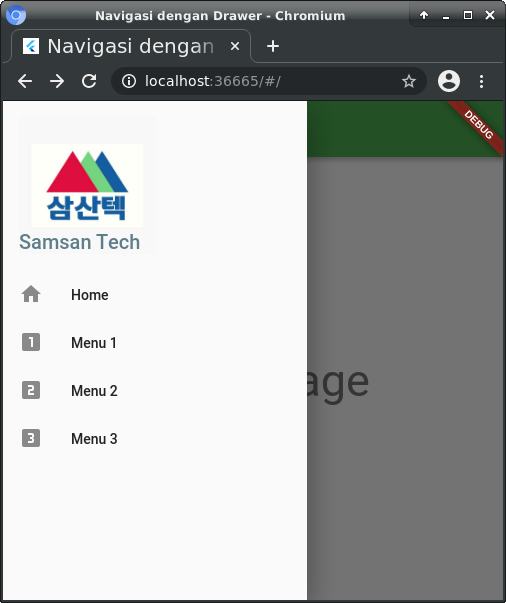
\includegraphics[scale=0.5]{images/navigasi_drawer_01.png}
\par}


\section{Navigasi dengan Tab}

Navigasi dengan tab memasangkan N tab dengan N widget. Ketika tab pertama ditekan
penggunakan akan melihat widget pertama, dan seterusnya.
Pemasangan ini dilakukan dengan menggunakan widget \txtinline{TabBar}, \txtinline{TabBarView},
dan \txtinline{TabBarController}.

Untuk \txtinline{TabBarController}, kita dapat menggunakan \txtinline{DefaultTabController}
dengan parameter jumlah tab yang diperlukan. Misalkan, kita ingin menggunakan tiga
tab:
\begin{dartcode}
Widget build(BuildContext context) {
  return DefaultTabController(
    length: 3,
    child: Scaffold(...),
  )
}
\end{dartcode}

\txtinline{TabBarView} adalah widget yang diperlukan untuk menampung widget yang
akan ditampilkan ketika pengguna mengakses suatu tab.
\begin{dartcode}
child: Scaffold(
  body: TabBarView(
    children: [
      WidgetA(),
      WidgetB(),
      WidgetC(),
    ]
  ),
),
\end{dartcode}

Untuk \txtinline{TabBar}, kita dapat menambahkannya pada suatu \txtinline{AppBar}.
Objek \txtinline{Tab} dapat menampung icon dan/atau teks, dan ditambahkan sebagai
properti \txtinline{tabs} pada \txtinline{TabBar}.
Misalnya kita ingin menambahkan tab yang akan tampil pada \txtinline{appBar}.
\begin{dartcode}
child: Scaffold(
  appBar: AppBar(
    title: Text('Navigasi Tab'),
    bottom: TabBar(
      tabs: [
        Tab(icon: Icons.looks_one, child: Text('Tab 1')),
        Tab(icon: Icons.looks_two, child: Text('Tab 2')),
        Tab(icon: Icons.looks_3, child: Text('Tab 3')),
      ],
    ),
  ),
),
\end{dartcode}

Kita juga menambahkan tab pada bagian bawah aplikasi:
\begin{dartcode}
child: Scaffold(
  // ...
  bottomNavigationBar: Material(
    color: Theme.of(context).colorScheme.primary,
    child: TabBar(
      tabs: [
        Tab(icon: Icons.looks_one, child: Text('Tab 1')),
        Tab(icon: Icons.looks_two, child: Text('Tab 2')),
        Tab(icon: Icons.looks_3, child: Text('Tab 3')),
      ]
    )
  ),
),
\end{dartcode}

Contoh program:

\begin{dartcode}
import 'package:flutter/material.dart';

void main() => runApp(MyApp());
  
class MyApp extends StatelessWidget {
  @override
  Widget build(BuildContext context) {
    return MaterialApp(
      title: 'Navigasi dengan Drawer',
      theme: ThemeData(primarySwatch: Colors.green),
      routes: {
        '/': (BuildContext ctx) => HomePage(),
      },
    );
  }
}
  
class HomePage extends StatelessWidget {
  @override
  Widget build(BuildContext context) {
    return DefaultTabController(
      length: 3,
      child: Scaffold(
        appBar: AppBar(
          title: const Text('Tab Navigation'),
          bottom: TabBar(tabs: const <Widget>[
            Tab(icon: Icon(Icons.looks_one), child: Text('Show 1')),
            Tab(icon: Icon(Icons.looks_two), child: Text('Show 2')),
            Tab(icon: Icon(Icons.looks_3), child: Text('Show 3')),
          ]),
        ),
        body: TabBarView(
          children: <Widget>[
            Widget1(),
            Widget2(),
            Widget3(),
          ],
        ),
        bottomNavigationBar: Material(
          color: Theme.of(context).colorScheme.primary,
          child: TabBar(tabs: const <Widget>[
            Tab(icon: Icon(Icons.looks_one), child: Text('Show A')),
            Tab(icon: Icon(Icons.looks_two), child: Text('Show B')),
            Tab(icon: Icon(Icons.looks_3), child: Text('Show C')),
          ]),
        ),
      ),
    );
  }
}

class Widget1 extends StatelessWidget {
  @override
  Widget build(BuildContext context) {
    return Center(
      child: Container(
          child:  Text(
        "I'm widget 1",
        style: Theme.of(context).textTheme.headline4,
      )),
    );
  }
}

// ... teruskan untuk Widget2 and Widget3
\end{dartcode}

Contoh tampilan:

{\center
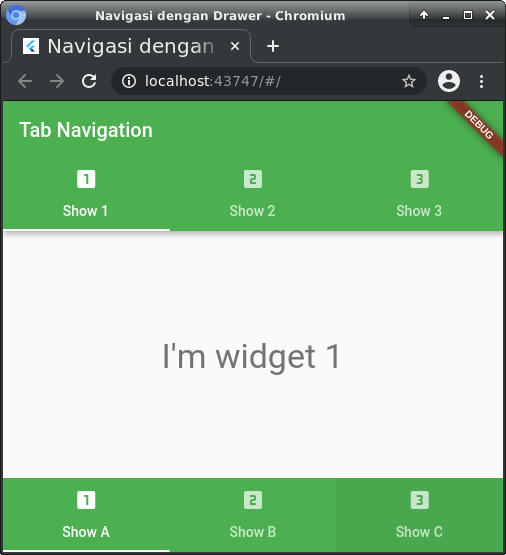
\includegraphics[scale=0.5]{images/navigation_tab_01.png}
\par}

\section{Dialog}

Dialog pada Flutter pada dasarnya adalah  suatu pop-up.
Pada Flutter kita dapat menggunakan metode \txtinline{showDialog()} untuk menampilkan
dialog. Fungsi ini dapat mengembalikan suatu \txtinline{AlertDialog} untuk menampilkan
suatu kotak dialog yang dapat menerima input dari user yang biasanya berupa respon
biner (yes or no). Untuk menerima respon dari pengguna, kita perlu mendefinisikan
callback sebagai \txtinline{async}.

\begin{dartcode}
import 'package:flutter/material.dart';

void main() => runApp(MyApp());
  
class MyApp extends StatelessWidget {
  @override
  Widget build(BuildContext context) {
    return MaterialApp(
      title: 'Navigasi dengan Drawer',
      theme: ThemeData(primarySwatch: Colors.green),
      routes: {
        '/': (BuildContext ctx) => HomePage(),
      },
    );
  }
}
  
class HomePage extends StatelessWidget {
  @override
  Widget build(BuildContext context) {
    return Scaffold(
      appBar: AppBar(
        title: const Text('Dialogs'),
      ),
      body: Center(
        child: Container(
          child: Column(
            mainAxisAlignment: MainAxisAlignment.spaceAround,
            children: <Widget>[
              Text(
                'Dialogs',
                style: Theme.of(context).textTheme.headline4,
              ),
              ElevatedButton(
                child: const Text('No response'),
                onPressed: () => showDialog<void>(
                  context: context,
                  builder: (BuildContext context) {
                    return AlertDialog(
                      content: const Text('Press OK to continue'),
                      actions: <Widget>[
                        FlatButton(
                            child: const Text('OK'),
                            onPressed: () => Navigator.pop(context)),
                      ],
                    );
                  },
                ),
              ),
              ElevatedButton(
                child: const Text('Get a response'),
                onPressed: () async {
                  final String response = await showDialog<String>(
                    context: context,
                    builder: (BuildContext context) {
                      return AlertDialog(
                        content: const Text('Are you sure?'),
                        actions: <Widget>[
                          FlatButton(
                              child: const Text('Yes'),
                              onPressed: () => Navigator.pop(context, 'Yes')),
                          FlatButton(
                              child: const Text('No'),
                              onPressed: () => Navigator.pop(context, 'No')),
                        ],
                      );
                    },
                  );
                  print('response = $response');
                },
              ),
            ],
          ),
        ),
      ),
    );
  }
}  
\end{dartcode}

Tampilan aplikasi ketika button ditekan:
{\center
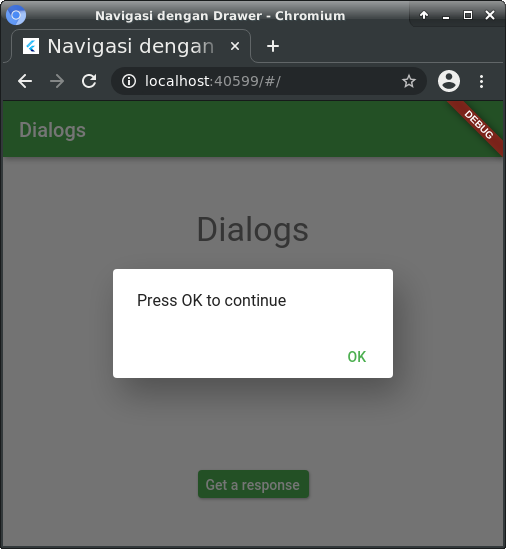
\includegraphics[scale=0.5]{images/navigation_dialog_2.png}%
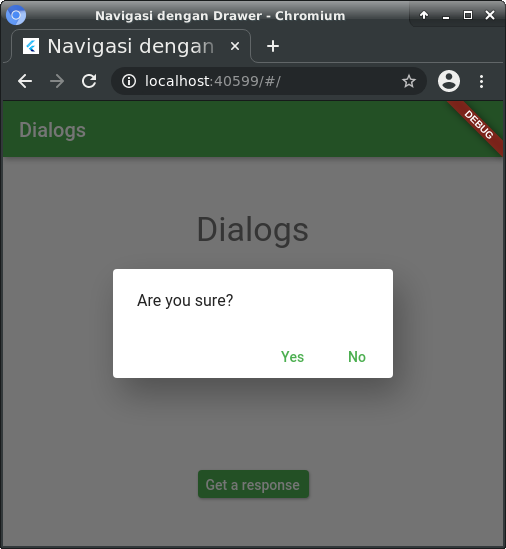
\includegraphics[scale=0.5]{images/navigation_dialog_3.png}
\par}


\section{Tugas (kelompok)}

Kombinasikan keempat contoh tersebut dalam satu aplikasi.
Program dapat dimodifikasi sesuai dengan dengan yang diinginkan.

\bibliographystyle{unsrt}
\bibliography{BIBLIO}




\end{document}
